\documentclass{article}
\usepackage{graphicx}
\usepackage{amsmath}
\usepackage{mathtools}
\usepackage[utf8]{inputenc}
\usepackage{changepage}
\providecommand{\abs}[1]{\lvert#1\rvert}
\providecommand{\norm}[1]{\lVert#1\rVert}
\usepackage{xcolor, colortbl}
\usepackage{array, multirow, multicol}
\usepackage{float}

\begin{document}
\begin{titlepage}
    \centering
    {
\includegraphics[width=2.5cm]{logo.png}\par}
    {\texttt{\bfseries \LARGE Universidad Nacional Autónoma de México} \par}
    \vspace{1cm}
    {\itshape \Large \bfseries Facultad de Estudios Superiores Acatlán \par}
    \vspace{3cm}
    {\scshape \Huge Ejercicio 1: Error de Redondeo \par}
    \vspace {3cm}
    {\slshape \Large Materia: Métodos Numéricos \par}
    \vspace{2cm}
    {\Large Autor: Díaz Valdez Fidel Gilberto\par}
    {\Large Número de cuenta: 320324280\par}
    \vfill
\end{titlepage}

\section{Propósito}
Aplicar los conceptos de error de redondeo para representar números de tipo flotante
por una computadora.

\section{Indicaciones}
1. Sea una computadora con: 
\begin{itemize}
    \item $B=2$
    \item 3 bits para el exponente (p)
    \item 5 bits para la mantisa (q)
    \item El rango de los posibles datos representados en el exponente con base en binario va desde
    1 a 7.
\end{itemize}

2. Sea una computadora con un tamaño de palabra de 12 bits y $B=2$, 1 bit del signo, 4 bits del
exponente y 7 bits de la mantisa.
\begin{itemize}
    \item  Determinar el rango del exponente.
    \item  Indicar los números más grande y más pequeño (en magnitud) que se pueden
    representar. En base 2 y base decimal.
\end{itemize}

3. Determinar el número que representa el siguiente número máquina, además de los números
anterior y posterior que pueden representarse. En base 2 y base decimal.

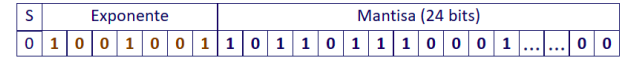
\includegraphics[width=0.8\linewidth]{Indicaciones.png}

\section{Ejecución}
\subsection{Primer Inciso}
Haciendo uso de la fórmula vista en clase para conocer el exponente de un dato
representado en binario se podrá conocer el rango del exponente y la fórmula es la
siguiente:

$-(B^p - 1 ) a\cdot2^p $
$-(2^3 - 1 ) a\cdot2^3 $

Por lo tanto el rango del exponente es el siguiente: $e \in [-3, 4]$. 

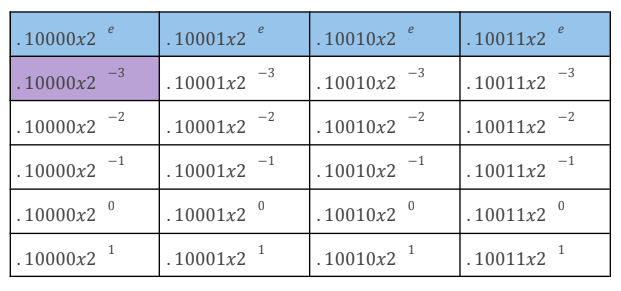
\includegraphics[width=1\linewidth]{Tabla1.png}
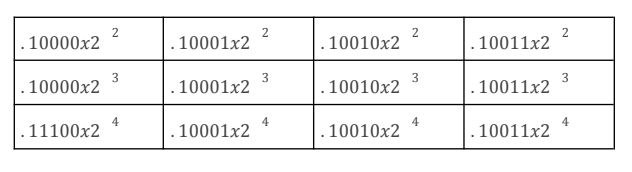
\includegraphics[width=1\linewidth]{Tabla2.png}
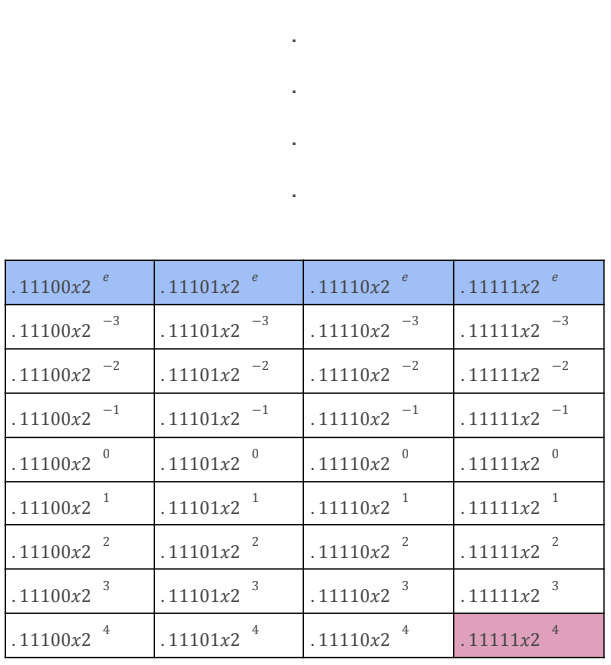
\includegraphics[width=1\linewidth]{Tabla3.png}
El mayor número posible para representar es: 0. 11111x$2^4$.
No tengo muy claro cual sería la manera correcta de convertir este número a
decimal, lo intente de la forma que vimos en clase sobre convertir un número binario 
normalizado a decimal, ya que ya tenía los datos necesarios como lo son el valor de
exponente y la mantisa, esta última sólo hacía falta convertir en decimal para poder
hacer uso de la fórmula de la siguiente manera:
$$(-1)^s B^e (1+f)$$
Donde sabemos que $s$ es el el valor del signo, $B$ la base, que en este caso
particular es 2, $e$ se trata del exponente que conocemos que es 4 y por último $f$
que es la parte fraccionaria o mantisa ya convertida en base decimal.

Haciendo uso de la fórmula queda de la siguiente manera:
$$(-1)^0 2^4(1 + 0. 96875) = 16. 96875$$

Pero también me parece pertinente comentar que si omito la parte de sumar un uno
en la operación o sea de la siguiente manera, el resultado es el siguiente:
$$(- 1)^0 2^4(0 + 0. 96875) = 15. 50$$

Por último, si convierto el número haciendo caso a el exponente por mi cuenta y
moviendo el punto de cifras significativas para después convertir ese número a
decimal según lo que sabemos que tiene valor al base binaria me da de resultado lo
siguiente:
$$0.11111\cdot2^4 = (1111. 1) = 1 + 2 + 4 + 8 + 0. 5 = 15. 5$$

Por lo siguiente no tengo muy claro cual es la mejor manera para poder convertir el
numero en cuestion a decimal a binario, usare la última manera ya que es la que
supongo y espero tenga mas sentido, llevo dias pensando en porque sucede esto
pero al no encontrar una respuesta clara decidÍ poner todo el proceso en la tarea, de
igual forma le llevaré mis dudas a mi profesora el respectivo día, otra de las razones
por las que lo haré de la última forma es porque realmente nunca se especifica si
este número en cuestión se trata de un número máquina normalizado (yo pense que
si, debido a que tenia las caracteristicas, pero la distinción tan grande entre
resultados me resulta preocupante). .

El mayor número posible para representar es: $0. 10000\cdot2^{-3}$
$$0. 10000x2^{-3} = (0. 00010000) = 0. 0625$$
El resultado tratándolo como un número normalizado binario es el siguiente:
$$(- 1)^0 2^{-3}(1 + 0. 5) = 0. 625$$

\subsection{Segundo Inciso}
El rango del exponente sabemos que se saca con la fórmula anterior vista:
$$-(B^p - 1 ) a\cdot2^p $$
$$-(2^3 - 1 ) a\cdot2^3 $$
$$-7 \rightarrow 8 $$
Por lo tanto: $e\in [-7,8]$
El número más pequeño para representar seria:
$$- 0. 1000000\cdot2^{-7}$$
Que en usando la fórmula sería en base decimal la siguiente:
$$(- 1)^1\cdot2^{-7}(0 + 0. 5) = 0. 01171875$$

Pero si se hace la misma operación sin sumar la unidad da de resultado lo siguiente:

$$(- 1)^1\cdot2^{-7}(1 + 0. 5) = 0. 00390625$$
En número binario representado y moviendo el punto acorde al valor del exponente
el número es el siguiente: 0. 00000001000000 = (0. 00390625)

Otra vez vuelvo a caer en el mismo escenario donde no estoy seguro de cual sea la
manera ideal para encontrar el valor decimal para el número binario dado, si usando
la fórmula que provoca un cambio drástico en el resultado o, por otro lado mover el punto del número según el exponente para así calcular el decimal que a su vez va a
coincidir con el resultado de la usar la formula pero omitiendo la parte de sumar una
unidad.

El número más grande para representar sería:
$$0. 1111111\cdot2^8$$
Usando la fórmula para un número normalizado máquina en binario a decimal sería:
$$(- 1)^0\cdot2^8(1 + 0. 9921875 ) = 510$$

Pero si se hace la misma operación sin sumar la unidad da de resultado lo siguiente:
$$(-1)^0\cdot2^8(0 + 0. 9921875 ) = 254$$

En número binario representado y moviendo el punto acorde al valor del exponente
el número es el siguiente:
$$11111110 = (2 + 4 + 8 + 16 + 32 + 64 + 128) = 254$$

Que de igual manera coincide con el resultado de la fórmula pero la fórmula que fue
cambiada para que no se sume una unidad. Con respecto a esto tengo varias dudas
ya que he realizado, para cotejar y comprobar cual es mi error o de dónde sale tanta
variación con respecto a los resultado, que es obvio que tiene que ver con esa
unidad que debe ser sumada en la fórmula, pero al realizar el mismo experimento
con los ejemplos que vimos en las diapositivas en clase me sucede lo mismo.

Al convertir el número máquina normalizado a decimal según la fórmula da un
resultado distinto al que mover el punto según el exponente y posterior a eso
calcular el valor de binario a decimal, pero curiosamente ese valor coincide con el
que saldría de aplicar la fórmula pero excluyendo el sumarle una unidad, como no
estoy seguro de cual sea la manera correcta por esto pongo las tres posibilidades
pero realmente me gustaria conocer el porque la diferencia y que significa.

\subsection{Tercer Inciso}
$$p = 7$$
$$q = 24$$
Exponente: 
$$c = (1001001) = 64 + 8 + 1 = 73$$
$$e = c - (2^{p1} - 1) = 73 - (63) = 10$$
Mantisa o parte fraccionaria:
$$101101110001... 0 = (\frac{1}{2})^-1 + (\frac{1}{2})^2+ (\frac{1}{2})^3 + (\frac{1}{2})^4 + (\frac{1}{2})^7 + (\frac{1}{2})^8 + (\frac{1}{2})^12 =0. 715087890625 $$

Haciendo uso de la fórmula que pondré a continuación el resultado es el siguiente:
$$(- 1)^0\cdot2^{10}(1 + 0. 715087890625) = 1756. 25$$

Lo siguiente que se debe hacer es convertir el número en base binaria pero creo
que aquí radica el problema que llevo planteando durante toda la tarea, para pasarlo
a base decimal y conocer su valor se hace uso de la fórmula antes escrita, pero
para regresarlo a base binaria no se si deberia ser lo mismo si se pasa a partir del
número que nos dan al principio con su mantisa y exponente que todo ya se
encuentra en base binaria y solo debería ser necesario recorrer el punto a que si se
pasa a binario el resultado final ya calculado con la fórmula. Tal vez ahí se
encuentre el problema, que en la forma normalizada aunque parezca estar ya en
base binaria, no lo es y por lo tanto no se puede recorrer el punto como nos lo
pediría el exponente. Sea cual sea la respuesta, lo convertiré en binario de ambas
formas.

En binario a partir del resultado de la fórmula:
$$11011011100. 01$$
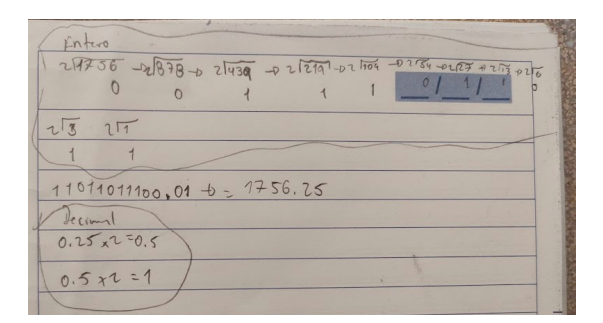
\includegraphics[width=1\linewidth]{Hoja1.png}
Así fue el cálculo para conocer su valor en binario.

En binario a partir del número en binario proporcionado en la mantisa y el
exponente:
$$1011011100. 010000... 0$$

Para conocer cúal es el valor inmediato posible de representar es necesario restarle
un dígito a la mantisa y el procedimiento fue el siguiente:

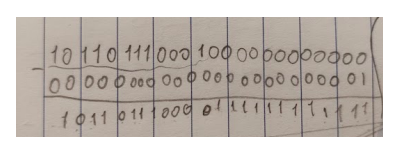
\includegraphics[width=1\linewidth]{Hoja2.png}

Conociendo el dato de la mantisa ahora solo será necesario conocer su valor en
base decimal para poder hacer uso de la fórmula, por lo que se calcula como
anteriormente:
Mantisa: 

$$10110111000011..... 1 = (\frac{1}{2})^1 + (\frac{1}{2})^3 + (\frac{1}{2})^4 + (\frac{1}{2})^6 + (\frac{1}{2})^7  + (\frac{1}{2})^8 + ... + (\frac{1}{2})^{24} = 0. 7150878310203552$$

Haciendo uso de la fórmula que pondré a continuación el resultado es el siguiente:
$$(- 1)^0\cdot2^{10}(1 + 0. 7150878310203552) = 1756. 2499389648437248$$

En binario a partir del resultado de la fórmula:
$$11011011100. 001111111$$

La parte entera no cambió pero como la decimal si, se procedió haciendo el cálculo
pero tras varias repeticiones y pruebas no parece ser corto o terminar de manera
rápida por lo que solo hice una aproximación.

En la calculadora iba haciendo la operación de multiplicar por dos la parte
fraccionaria para poder conocer la parte fraccionaria en binario, pero como no
parecía tener final pronto el procedimiento decidí dejarlo ahí.

En binario a partir del número en binario proporcionado por la mantisa y el
exponente:
$$1011011100. 00111... 111$$
Por último para conocer cúal es el siguiente dato posible para representa solo es
necesario sumar un dígito a la mantisa teniendo como resultado una mantisa de la
siguiente forma:
$$101101110001.. 001$$

Conociendo el dato de la mantisa ahora solo será necesario conocer su valor en
base decimal para poder hacer uso de la fórmula, por lo que se calcula como
anteriormente:

Mantisa: 
$$101101110001.. 001 = (\frac{1}{2})^1 + (\frac{1}{2})^3+ (\frac{1}{2})^4+ (\frac{1}{2})^6+ (\frac{1}{2})^7+ (\frac{1}{2})^8+ (\frac{1}{2})^{12}+ (\frac{1}{2})^{24} = 0. 7150879502296448$$

Haciendo uso de la fórmula que pondré a continuación el resultado es el siguiente:

$$(- 1)^0\cdot2^{10}(1 + 0. 7150879502296448) = 1756. 2500610351562752$$

En binario a partir del resultado de la fórmula:
$$11011011100. 01000000000001$$

Lo mismo que en el caso anterior, no parecía tener final el cálculo para encontrar la
parte fraccionaria en binaria, al menos no de manera rápida, pero eso fue una
aproximación bastante satisfactoria creo yo.

Aquí sucedió lo mismo que en el binario anterior del número más próximo menor,
hice el procedimiento en calculadora y solo iba anotando el resultado pero de igual
manera no parecía tener un final cercano.

En binario a partir del número en binario proporcionado por la mantisa y el
exponente:
$$1011011100. 01.... 001$$

\section{Conclusión}
Por último expondré una foto de mi hoja de ideas sobre cómo primero desarrolle
varias veces las ideas para después sintetizar y plasmarlas en este documento.

Asi se terminara este último inciso y a su vez
llega a su fin la tarea de error de redondeo,
espero no contenga muchos errores, gracias
por su atención.

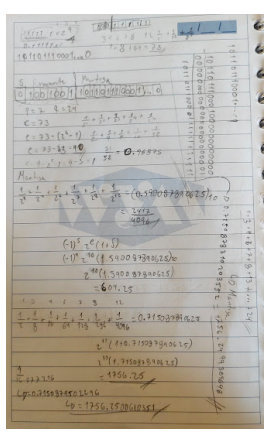
\includegraphics[width=1\linewidth]{Hoja5.png}




%[width=1\linewidth]
\end{document}